\section{Deutsch und Kommunikation}


%%% Anfang: tl;dr
\subsection{tl;dr - Zusammenfassung der Zusammenfassung}

%%% Ende: tl;dr
%%%%%%%%%%%%%%%%%%%%%%%%%%%%%%%%%%%%%%%%%%%%%%%%%%%%%%%%%%%%%%%%%%%%%%%%%%%%%%%%

%%% Anfang: Lernen
\subsection{Lernen}

In den folgenden Abschnitten werden wir uns mit den Voraussetzungen und Erfolgsfaktoren des Lernens beschäftigen.

%%% Anfang: Lernen > Physiologie
\subsubsection{Physiologische Voraussetzungen des Lernerfolges}

\paragraph{Aufbau des Gehirns}~\\
\\
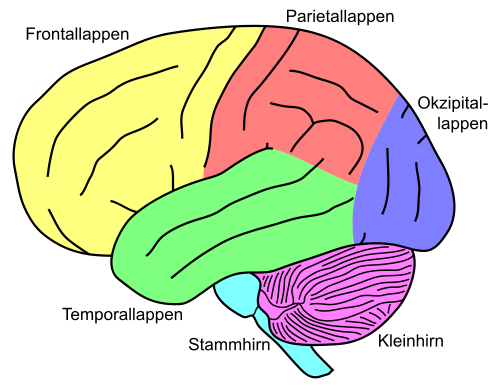
\includegraphics[scale=0.7]{1jahr_pictures/dko-pic/dko-gehirnaufbau.png}~\\
\\
Der {\bf Parietallappen} (auch Scheitellappen genannt) ist für die Integration sensorischer Informationen zuständig. Im vorderen Teil wird die haptische Wahrnehmung (Berührung, Druck, Vibration, Temperatur und teilweise auch Schmerz) verarbeitet. Der obere Teil hingegen ist zuständig für die visuelle Bewegungssteuerung und die Erkennung von Reizen im betrachterbezogenen Raum. Somit ermöglicht dieser Teil des Gehirns die räumliche Aufmerksamkeit. Im unteren Teil des Parietallappens finden das räumliche Denken und \ql quasi-räumliche\qr\ Prozesse wie Rechnen und Lesen statt.\\
\\
Im {\bf Okzipitallappen} (auch Hinterhauptlappen genannt), befinden sich die primäre und die sekundäre Sehrinde. In der primären Sehrinde werden die Signale der Netzhaut verarbeitet. Die sekundäre Sehrinde dient dem Gehirn als Assoziationszentrum. Sie stellt die Verarbeiteten Muster aus der primären Sehrinde bekannten Sinneseindrücken gegenüber, interpretiert und erkennt sie. Zudem stellt sie eine Verknüpfung mit anderen Rindenarealen des Großhirns dar.\\
\\
Im {\bf Kleinhirn} wird die Feinsteuerung der Motorik vorgenommen. Beim implizierten Lernen (unbewusste oder spielerische Aneignung von Fertigkeiten und Wissen beim Ausüben einer Tätigkeit) spielt es eine große Rolle, da es die automatisierten Tätigkeiten speichert.\\
\\
Das {\bf Stammhirn} besteht aus dem {\it verlängerten Rückenmark}, der {\it Brücke} und dem {\it Mittelhirn}. Das verlängerte Rückenmark hat eine Schlüsselposition im Nervensystem des Körpers. Alle Nervenbahnen, die das Gehirn mit dem Körper verbinden, fließen durch das verlängerte Rückenmark. Zusätzlich ist es für die Kontrolle des Blutkreis und der Atmung zuständig. So befinden sich zum Beispiel die Rezeptoren zur Steuerung des Atemreflexes dort. Weitere wichtige Reflexe, die aus dem verlängerten Rückenmark gesteuert werden sind Nies-, Husten-, Schluck- und Saugreflex sowie das Erbrechen. \\
Die Brücke dient als Durchgangsstation für alle Nervenfasern zwischen den vorderen und dahinterliegenden Abschnitten des Zentralnervensystems sowie als Umschaltstation zwischen dem Großhirn und dem Kleinhirn.\\
Das Mittelhirn steuert die Augenmuskulatur und leitet die Erregungen sensibler Nerven an das Großhirn weiter.\\
\\
Der {\bf Temporallappen} (Schläfenlappen) ist für die Verarbeitung der akustischen Signale zuständig. In ihm befindet sich auch das {\it sensorische Sprachzentrum}, welches für das Sprachverständnis wichtig ist. Weiterhin wird hier auch das visuelle Arbeitsgedächtnis lokalisiert, was der kurzen Speicherung von aktuellen Wahrnehmungen dient. Auch der Vergleich mit den nächstfolgenden Wahrnehmungsinhalten und das Erkennen von komplexen nichträumlichen auditorischen und visuellen Reizen (z.B. das Erkennen von Gesichtern) findet im Temporallappen statt.\\
\\
Im {\bf Stirnhirn} findet die Steuerung der Bewegungen sowie das Auswählen von Bedingungen für diese Bewegungen statt. Die kognitiven Prozesse werden hier reguliert um eine situationsgerechte Ausführung von Handlungen sicherzustellen. Im Stirnhirn befindet sich auch das motorische Sprachzentrum, welches die Motorik zur Produktion der Sprache steuert.\\
\paragraph{Das Nervensystem}~\\
\\
Das menschliche Nervensystem besteht aus hochspezialisierten einzelnen Zellen({\it Neuronen}). Diese Zellen können sich jedoch nicht mehr teilen, weshalb Verletzungen im Nervensystem nicht heilen können. Die Zellen sind untereinander verbunden (ein neugeborenes Kind hat ca. 50 Billionen Verbindungen zwischen den Nervenzellen) und senden Signale aus, sobald die Summe der Eingangssignale einen Bestimmten Schwellenwert überschreitet. Eine Einteilung des Nervensystems kann nach verschiedenen Kriterien erfolgen. Für den Lernprozess ist allerdings die Klassifizierung in das vegetative und das somatische Nervensystem am wichtigsten.\\
Das {\bf vegetative Nervensystem} (Autonomes Nervensystem) ist der willentlichen Kontrolle weitestgehend entzogen. Es dient der Steuerung der inneren Organe.\\
Das {\bf somatische Nervensystem} (willkürliches oder animalisches Nervensystem) dient der Wahrnehmung von Umweltreizen und Reizen aus dem Körperinneren sowie der Steuerung der dem Bewusstsein und dem Willen unterworfenen Vorgängen. Dies impliziert bewusste ebenso wie willkürliche Bewegungen.\\

\paragraph{Lernprozesse}~\\
\\
Alles Prozesse des Lernens und der Gehirnentwicklung basieren auf einem Wachstum bzw. einer Veränderung der Verbindungen zwischen den weitgehend zufällig organisierten Neuronen. Das Lernen aktiviert eine Anzahl miteinander verknüpfter Nervenzellen. Diese Verbindung wird nach und nach zu einem \ql neuronalen Netzwerk\qr\ verstärkt, welches mit steigender Wiederholung des Lernprozesses immer besser und leichter aktivierbar wird. Dieses {\it synaptische Lernen} bedarf somit vieler Wiederholungen, weswegen häufiges Lernen wirksamer als einmaliges längeres Lernen ist.\\
Das {\it limbische System} (bestehend u.a. aus dem Hippocampus und der Amygdala) liefert eine emotionale Bewertung der aufgenommenen Informationen. Je besser diese Bewertung ist, desto besser wird die Übertragung dieser Information in das Langzeitgedächtnis. Der Hippocampus erfüllt hierbei eine Türsteherfunktion. Bei einer mehrfachen Wiederholung der gleichen Information \ql schließt er die Tür\qr . Daraus folgt, dass Abwechslung einen besseren Lerneffekt erzielt. Wird z. B. ein englischer Satz in verschiedenen Satzstellungen gelernt, so blockiert der Hippocampus nicht und es wird ein Lerneffekt erzielt. Dieser Effekt kann sogar schon durch Aussprache in einer anderen Stimmlage erreicht werden.\\
Da während des Schlafes eine starke Kommunikation zwischen dem Hippocampus und der Großhirnrinde stattfindet, wird davon ausgegangen, dass die frischen Eindrücke vornehmlich während des Tiefschlafs aus dem Hippocampus in die Großhirnrinde übertragen werden.\\
Eine zweite Überprüfungsstelle ist die Amygdala. Sie überprüft alle im Gehirn eingehenden Sinneswahrnehmungen. Erkennt die Amygdala Gefahr oder Unheil, so mobilisiert sie Abwehr. Da auch unbewusste Erinnerungen direkt in der Amygdala gespeichert werden können, wird die Angst beim Lernen unter Angst direkt mit gelernt. Wird eine Assoziation zu diesen Erinnerungen geweckt, so wird von der Amygdala der Körperzustand wieder hergestellt, welcher beim Speichern des ursprünglichen Ereignisses geherrscht hat. Da das Lernen unter Angst die Angst somit noch verstärkt, folgt als Konsequenz für das Lernen: {\bf Lernen ist nur in guter emotionaler Atmosphäre effektiv!}\\

\paragraph{Neurokognitive Effekte durch Sport}~\\
\\
Bei einer körperlichen Belastung kommt es zu einer Verlagerung der Gehirnaktivität aus der Großhirnrinde heraus in die Bewegungszentren und den Hirnstamm. Die Gehirnleistung wird zur Sicherstellung der lebenswichtigen Funktionen sowie der Steuerung der Bewegungsabläufe dort benötigt. Dadurch ist bei hoher körperlicher Belastung kein Lernen mehr möglich, da den für das Lernen wichtigen Gehirnarealen keine Leistung mehr zur Verfügung steht.\\
Durch die Verlagerung der Gehirnaktivität kommt die Gehirnaktivität im vorderen Teil des Stirnlappens, welcher für das Arbeitsgedächtnis sowie das exekutive Handeln zuständig ist, fast vollständig zum erliegen. Dieser Effekt ist in etwa wie der eines Computerneustarts, nach dem Sport kann mit einem frischen und aufnahmefähigen Gehirn weitergelernt werden.\\
Funktionieren tut der Effekt jedoch nur bei positiven Emotionen beim Sport, da sonst die Amygdala den Sport mit negativen Emotionen verbindet und sich auch nach dem Sport noch in einem Abwehrzustand befindet, welcher die Inhalte abblockt. Zum erreichen des Effektes reichen auch kurze Bewegungspausen von fünf bis zehn Minuten.\\

%%% Anfang: Lernen > Typen
\subsubsection{Welche Lerntypen gibt es?}

\paragraph{Visueller Lerntyp}~\\
\paragraph{Haptischer Lerntyp}~\\
\paragraph{Auditiver Lerntyp}~\\
\paragraph{Kommunikativer Lerntyp}~\\

%%% Anfang: Lernen > Methoden
\subsubsection{Lernmethoden}

Lernen ist eine angeborene Fähigkeit, die durch Lernmethoden verbessert, vereinfacht und intensiver gestalten werden kann. Lernmethoden sind Methoden, Werkzeuge bzw. Hilfsmittel, mit denen effizienter lernen kann, um so Wissen und Fähigkeiten zu erlangen. Folgend sind 10 Methoden und ihr jeweiliger Nutzen aufgeführt.

{\bf 10 Lernmethoden}\\
\begin{enumerate}
	\item Markieren: Das Unterstreichen ist zugleich eine der wichtigsten Lernmethoden und auch noch sehr einfach. Man hebt schlicht und einfach die wichtigsten Teile des Textes mit verschiedenen Farben hervor. Idealerweise sollte man den Text vorher einmal komplett lesen und verstanden haben, bevor man ihn unterstreicht und zum Lernen benutzt.
	\item Notizen: Zusammen mit dem Unterstreichen gehören Notizen zu den weit verbreiteten Lernmethoden. Indem du das Wichtigste in deinen eigenen Worten aufschreibst wirst, du es besser im Kopf behalten können. Dabei kommt es darauf an, den Inhalt so weit wie möglich zu reduzieren, ohne dabei die Kernpunkte auszulassen.  Man kann Notizen traditionell mit Stift und Papier erstellen, oder aber man greift auf Tools zurück.
	\item Mindmap: Eine Mindmap, auch Gedanken(land)karte genannt, die man z.B. zum Erschließen und visuellen Darstellen eines Themengebietes, zum Planen oder für Mitschriften nutzen kann. Hierbei soll das Prinzip der Assoziation helfen, Gedanken frei zu entfalten und die Fähigkeit des Gehirns zur Kategorienbildung zu nutzen. Die Mind-Map wird nach bestimmten Regeln erstellt und gelesen. Den Prozess bzw. das Themengebiet bzw. die Technik bezeichnet man als Mind-Mapping.
	\item Karteikarten: Eine besonders effektive Lernmethode, wenn es darum geht, Fakten, Daten, Zahlen oder Vokabeln zu verinnerlichen. Das Lernen von Themen fällt somit wesentlich leichter. Außerdem macht es auch mehr Spaß mit Karteikarten zu lernen.
	\item Case Studies: Um den Unterricht der Jugendlichen- wie der Erwachsenenbildung zu bereichern, werden häufig Fallstudien eingesetzt. 
Die Lösung wird dabei in der Regel offen gelassen, die Lernenden sollen selbst ein plausibles Ergebnis erarbeiten. 
Auch gibt es Fallstudien, welche die Lösung mitliefern und die Lernenden zur Diskussion darüber und zur Suche nach Alternativen ermuntern sollen.  Eine Fallstudie (Fall, Case, Case Study) ist daher eine für Unterrichtszwecke erstellte Schilderung einer Situation und ihrer Einflussfaktoren, welche sowohl die aktive Auseinandersetzung mit dem Inhalt als auch konkretes Handeln des Lernenden bezweckt.
	\item Tests: Tests sind eine hervorragende Lernmethode, um dein Wissen zu überprüfen. 
Du kannst die Bereiche herausfinden, in denen du bereits gut bist und wo du eventuell noch Nachholbedarf hast. Darüber hinaus könnt ihr euch mit Freunden gegenseitig testen und dabei herausfinden, welche wichtigen Details man übersehen hat. Daher empfehlen wir, Tests vor Prüfungen zu erstellen und sie mit Freunden auszutauschen.
	\item Brainstorming: Auch diese Lernmethode kann in einer Gruppe durchgeführt werden. 
Beim Brainstorming sammelt eine Gruppe von Leuten Ideen zu einem bestimmten Thema. Der Vorteil einer Gruppe ist, dass auch andere Ideen und Perspektiven berücksichtigt werden. Bei der Prüfungsvorbereitung kann man gemeinsam spezifische Fragen beantworten und so die Materie besser verstehen.
	\item Eselsbrücke: Eselsbrücken sind vor allem dazu geeignet, sich Listen oder Kategorien von Informationen zu merken. Sie funktionieren so gut, weil man sich entweder unbekannte Konzepte dadurch merkt, dass man sie mit bereits bekannten Konzepten in Verbindung bringt, oder weil ein Reim eingebunden ist.
	\item Zeichnungen: Viele Leute haben ein gutes visuelles Gedächtnis, sodass sie sich Informationen besser merken können, wenn sie mit einem bestimmten Bild oder einer Zeichnung assoziieren. Beim Lernen kann man von dieser Eigenschaft Gebrauch machen.
\end{enumerate} 

%%% Anfang: Lernen > Faktoren
\subsubsection{Äußere Einflussfaktoren auf den Lernerfolg}
\paragraph{Einfluss der direkten Umgebung}~\\
\paragraph{Einfluss des sozialen Umfeldes}~\\
\paragraph{Einfluss der Ernährung}~\\
Das Gehirn kann im Gegensatz zum Rest des Körpers nur mit Glukose umgehen. Generell gilt, je höher der Glukosespiegel ist, desto besser können wir uns konzentrieren und desto besser ist unsere geistige Leistungsfähigkeit. Jedoch gibt es ein oberes Limit, ab dem der Körper vermehrt Insulin produziert, welches den Glukosespiegel rapide sinken lässt. Es folgen Müdigkeit, Konzentrationsstörungen und generell eine geringere Leistungsfähigkeit. Statt stark zuckerhaltige Lebensmittel zu verzehren, sollten also Lebensmitteln mit einem hohen Anteil an komplexen Kohlenhydraten bevorzugt werden, damit der Glukosespiegel nicht zu schnell steigt und über einen längeren Zeitraum konstant bleibt.
Konzentrationsschwäche kann aber auch dann auftreten, wenn dem Körper bestimmte Mineralien fehlen wie bspw. Eisen. Für optimale Leistungsfähigkeit sollte auf eine gesunde Ernährung geachtet werden.
\paragraph{Einfluss von Drogen}~\\
Koffein
%%% Ende: Lernen
%%%%%%%%%%%%%%%%%%%%%%%%%%%%%%%%%%%%%%%%%%%%%%%%%%%%%%%%%%%%%%%%%%%%%%%%%%%%%%%%

%%% Anfang: Kommunikation
\subsection{Das 4-Ohren-Modell}
Das 4-Ohrenmodell wurde von Schulze von Thun im [Jahr] entwickelt. Es basiert auf der Beobachtung, dass [Ampel]. Um solche Situationen zu erklären, führt von Thun vier Aspekte bzw. vier Ohren ein:

\begin{tabular}{ll}
{\bf Ebene} & {\bf Beispiel: Die Ampel ist grün.}\\
Sachebene & Die Ampel ist grün (nicht rot).\\
Beziehungsebene & Du bist kein guter Autofahrer.\\
Selbstoffenbarungsebene & Ich bin ungeduldig.\\
Appellebene & Fahr schneller!\\
\end{tabular}

[BILD?]\\

Die verschiedenen Ebenen zeichnen sich durch verschiedene Elemente aus. Die Sachebene stellt eine Feststellung dar, die Beziehungsebene sagt etwas über die beteiligten Personen bzw. etwas über das Gegenüber aus. Im Gegenzug zeichnet sich die Selbstoffenbarungsebene durch Aussagen über die eigene Person aus und die Appellebene stellt in der Regel einen Ausruf dar.

Im therapeutischen Kontext wird empfohlen, sich auf Sach- und Selbstoffenbarungsebene zu bewegen, damit sich das Gegenüber nicht in seinem Charakter kritisiert führt.

%%% Ende: Kommunikation
%%%%%%%%%%%%%%%%%%%%%%%%%%%%%%%%%%%%%%%%%%%%%%%%%%%%%%%%%%%%%%%%%%%%%%%%%%%%%%%%